\documentclass[10pt]{article}

\usepackage{amsmath}
\usepackage{amssymb}
\usepackage{array}
\usepackage{tabu}
\usepackage{lmodern}
\usepackage{graphicx}
\usepackage[space]{grffile}
\usepackage{subfigure}
\usepackage{longtable}
\usepackage{multirow}
\usepackage[margin=1.0in]{geometry}
\renewcommand{\baselinestretch}{2.0}

%\usepackage[font=small,labelfont=bf,labelsep=period]{caption}
\usepackage[style=authoryear,sorting=nyt,url=false,isbn=false,doi=false,firstinits=true,backend=biber]{biblatex}

\renewcommand{\baselinestretch}{2.0}
\renewcommand*\contentsname{Table of Contents}
%\captionsetup{font={stretch=2.0}}

\DeclareNameAlias{default}{last-first}

\DefineBibliographyStrings{english}{%
	andothers = {\addcomma\addspace\textsc{et\addabbrvspace al}\adddot},
	and = {\textsc{and}}
}
\renewcommand*{\labelnamepunct}{\space\space}

\renewbibmacro{in:}
{%
	\ifentrytype{article}{%
	}{%
		\printtext{\bibstring{in}\intitlepunct}%
	}%
}
\renewbibmacro*{volume+number}{%
	\printfield{volume}%
	\setunit*{\addcomma\space}%
	\printfield{number}%
	\setunit{\addcomma\space}}

\DeclareFieldFormat{pages}{#1}

\renewbibmacro*{publisher+location+date}{%
	\printlist{publisher}%
	\setunit*{\addcomma\space}%
	\printlist{location}%
	\setunit*{\addcomma\space}%
	\usebibmacro{date}%
	\newunit}

\renewcommand{\newunitpunct}{\addcomma\space}
\DeclareFieldFormat[article,inbook,incollection,inproceedings,patent,thesis,unpublished]{title}{#1} 
\DeclareFieldFormat{year}{#1} 

\addbibresource{refs/ident_refs.bib}

\begin{document}
	\section{Introduction:}
	\subsection{Identifiability analysis: Definitions and Formulations}
	Any nonlinear dynamical system can be represented by a set of states $\mathbf{x}$, observables $\mathbf{y}$ that are dependent on the states, parameters $\mathbf{\mu}$, and inputs $u$ as in Equation (\ref{eq:dynmodel}). 
	\begin{subequations}\label{eq:dynmodel}
		\begin{align}
		\dot{\mathbf{x}} = g(\mathbf{x},\mathbf{\mu},u)\\
		\mathbf{y} = h(\mathbf{x},\mathbf{\mu},u)
		\end{align}
	\end{subequations}
	Identifiability concerns with the ability to determine a unique solution to the problem of estimating parameters $\mathbf{\mu}$ from given data on the system observables $\mathbf{y}$ for inputs $u$ \parencite{McLean2012}.	The identifiability of parameters in nonlinear models of physical processes can be classified into two categories: structural and practical identifiability. 
	
	Any system (Equation \ref{eq:dynmodel}) is said to be structurally or a priori identifiable if, for an input-output mapping defined by $\mathbf{y} = \Phi(\mu,u)$ for at least one input function $u$, any two values of parameters $\mathbf{\mu}_1$ and $\mathbf{\mu}_2$ satisfy the relationship in Equation (\ref{eq:stident}) below.
	\begin{align}\label{eq:stident}
	\Phi(\mathbf{\mu}_1,u) = \Phi(\mathbf{\mu}_2,u) \iff \mathbf{\mu}_1 = \mathbf{\mu}_2
	\end{align}
	Accordingly, any system that has an infinite number of solutions to the parameter estimation problem for all input functions is said to structurally non-identifiable. The effect of model structure and parameterization on the ability to infer true parameter values from experimental data is determined by the structural identifiability of the parameter. 
	
	When parameters are estimated on the basis of noisy data, the ability to estimate unique parameter values to satisfy Equation (\ref{eq:stident}) is referred to as practical identifiability. The effect of the available experimental data on the ability to estimate unique parameter values is determined by the practical identifiability of the parameter. Accordingly, practical identifiability of a parameter is contingent upon the nature, quality and quantity of data available to estimate the parameter as opposed to the structure and parameterization of the model. 
	%Thus, the identifiability of parameters in nonlinear models is dependent on the model structure, parameterization, and the quality and quantity of experimental data that is available for the purpose of estimation. 
	Thus, on the one hand, establishing the structural identifiability of parameters enables one to propose models that are not only appropriate representations of physical processes, but also are parameterized in such a way that the value of these parameters can be estimated. On the other hand, establishing practical identifiability of parameters in any model helps design experiments that are minimal, informative and useful for parameter estimation.
	
	\section{Methods:}
	 We use a profile likelihood-based approach \parencite{Raue2009a} to establish structural and practical identifiability of parameters in nonlinear kinetic models of metabolism. Briefly, the approach seeks to establish the existence/non-existence of bounds in confidence intervals for the estimates of parameters in nonlinear models. The profile likelihood is calculated based on Equation (\ref{eq:pl}) for each parameter $\theta_i$ where $\chi^2(\theta_i)$ is given by Equation (\ref{eq:chi2}).
	 \begin{align}\label{eq:pl}
	 \chi_{PL}^2(\theta_i) = \underset{\theta_{j\ne i}}{\mathrm{min}} \left[\chi^2(\theta)\right]
	 \end{align}
	 \begin{align}\label{eq:chi2}
	 \chi^2(\theta) = \sum_{k=1}^{m}\sum_{l=1}^{d}\left(\frac{y_{kl}^*-y_{kl}}{\sigma_{kl}^*}\right)^2
	 \end{align}
	 In the minimization objective shown in Equation (\ref{eq:chi2}) for parameter estimation, $y_{kl}^*$ is the available experimental time course data for each observable state $k$ at each $l$ time point. The difference between the data and the model estimates at these time points, $y_{kl}$ is weighted by the variance in the experimental data $\sigma_{kl}^*$. An algorithm to calculate the profile likelihood, $\chi_{PL}^2(\theta_i)$, based on Equation \ref{eq:pl} is given below.
	 
	 The identifiability of parameters is established through the confidence intervals of their estimates, $\left[\sigma_{i}^-,\sigma_{i}^+\right]$. The likelihood-based confidence interval for any parameter whose profile likelihood is estimated can be written on the basis of a threshold $\Delta_{\alpha}$ in the likelihood as in Equation (\ref{eq:pleci}).
	 \begin{align}\label{eq:pleci}
	 \{\theta|\chi^2(\theta)-\chi^2(\hat{\theta})<\Delta_{\alpha}\}
	 \end{align}
	 The threshold $\Delta_{\alpha}$ in the likelihood is the 1-$\alpha$ quantile of the $\chi^2$ distribution, represented as $\chi^2(\alpha,df)$. The confidence intervals obtained hold for $df$ degrees of freedom. For a choice of $df$=1 the confidence intervals will hold for each parameter individually, and confidence intervals that hold jointly for all parameters can be obtained by choosing the number of parameters as $df$. 
	
	The visualization of structurally and practically non-identifiable parameters using the profile likelihood approach is illustrated in Figure \ref{fig:identtypes}. The points of intersection between the profile likelihood curves (solid line) with the one parameter likelihood threshold ($\Delta_{\alpha} = \chi^2(\alpha,1)$, dashed line) provide the confidence intervals of the parameter $\theta_i$. The confidence intervals of a structurally non-identifiable parameter are unbounded, i.e., $\left[-\infty, +\infty\right]$ (Figure \ref{fig:identtypes}a), while the confidence intervals of a practically non-identifiable parameter are unbounded in at least one direction, i.e., $\left[\sigma_{i}^-,\sigma_{i}^+\right]$ where either $\sigma_{i}^- = -\infty$ or $\sigma_{i}^+ = +\infty$ (Figure \ref{fig:identtypes}b). If a parameter's estimates have a finite confidence interval then the parameter is said to be identifiable (Figure \ref{fig:identtypes}c). Note that the horizontal dotted lines in Figure \ref{fig:identtypes} represent the confidence interval thresholds ($\Delta_{\alpha}$) that are used to establish identifiability.
	
	\begin{figure}[!tbhp]
		\centering{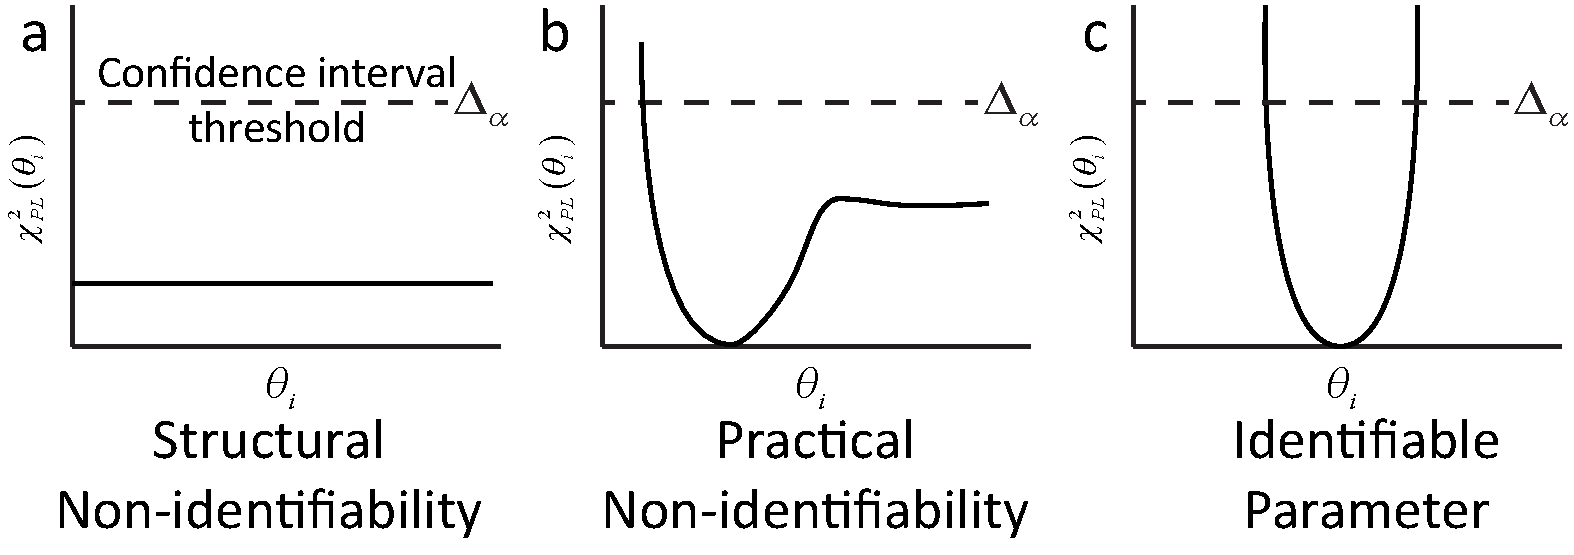
\includegraphics[width=.8\textwidth,height=.8\textheight,keepaspectratio]{figures/identifiability}}
		\caption{The profile likelihood estimates of a) a structurally non-identifiable, b) a practically non-identifiable and c) an identifiable parameter. The horizontal axis represents the changes in the value of the parameter ($\theta_i$) whose identifiability is being determined and the profile likelihood ($\chi^2_{PL}(\theta_i)$) is shown in the vertical axis. The confidence interval threshold ($\Delta_{\alpha}$) used to determine the identifiability of the parameter is denoted by the horizontal dotted line. Identifiable parameters are distinguished from non-identifiable parameters by the presence of both upper and lower bounds on their confidence interval estimates $\left[\sigma_{i}^-,\sigma_{i}^+\right]$. }\label{fig:identtypes}
	\end{figure}
	
	\subsection{Algorithm to calculate profile likelihood:}		
	\begin{enumerate}
		\item Start by solving the numerical optimization problem in Equation \ref{eq:pl} for a fixed value of $\theta_i$ to determine the initial point on the profile likelihood curve.
		\item Take an increasing/decreasing step $\theta_{step}$ in the direction of $\theta_i$.\\
		The increasing/decreasing steps in $\theta_i$ can be adapted to the shape of the profile likelihood curve that is encountered while running the algorithm. Accordingly, the step $\theta_{step}$ should satisfy Equation (\ref{eq:adaptivestep}) below, where $\theta^{k-1}$ refers to parameter estimates obtained from iteration $k-1$ of the above algorithm and $q\in \left[0,1\right]$.
		\begin{align}\label{eq:adaptivestep}
		\chi^2\left(\theta^{k-1}+\theta_{step}\right) - \chi^2(\theta^{k-1}) \approx q.\Delta_{\alpha}
		\end{align}
		\item Re-optimize $\theta_{j\ne i}$ using Equation \ref{eq:pl}.
		\item Repeat the last two steps until a desired threshold $\Delta_{\alpha}$ is exceeded or a maximal amount of steps is reached.
	\end{enumerate}
	
	Due to the dependence of practical parameter identifiability on the experimental data, the profile likelihood approach can be used to design experiments in such a way that the observables that are derived from these experiments can improve the practical identifiability of the parameters. We show how experimental design can have a meaningful impact on parameter identification and estimation in Figure \ref{fig:edwithpl}.	Assuming a parameter $\theta_i$ is practically non-identifiable (Figure \ref{fig:edwithpl}a), performing a profile-likelihood based identifiability analysis using simulated data can help determine the nature of experiments needed to make the parameter identifiable (Figure \ref{fig:edwithpl}b). In contrast, performing non-informative experiments without prior knowledge on their ability to change the identifiability of the parameter may provide data that cannot be used to estimate parameter $\theta_i$ (Figure \ref{fig:edwithpl}c).
	 
	\begin{figure}[!tbhp]
		\centering{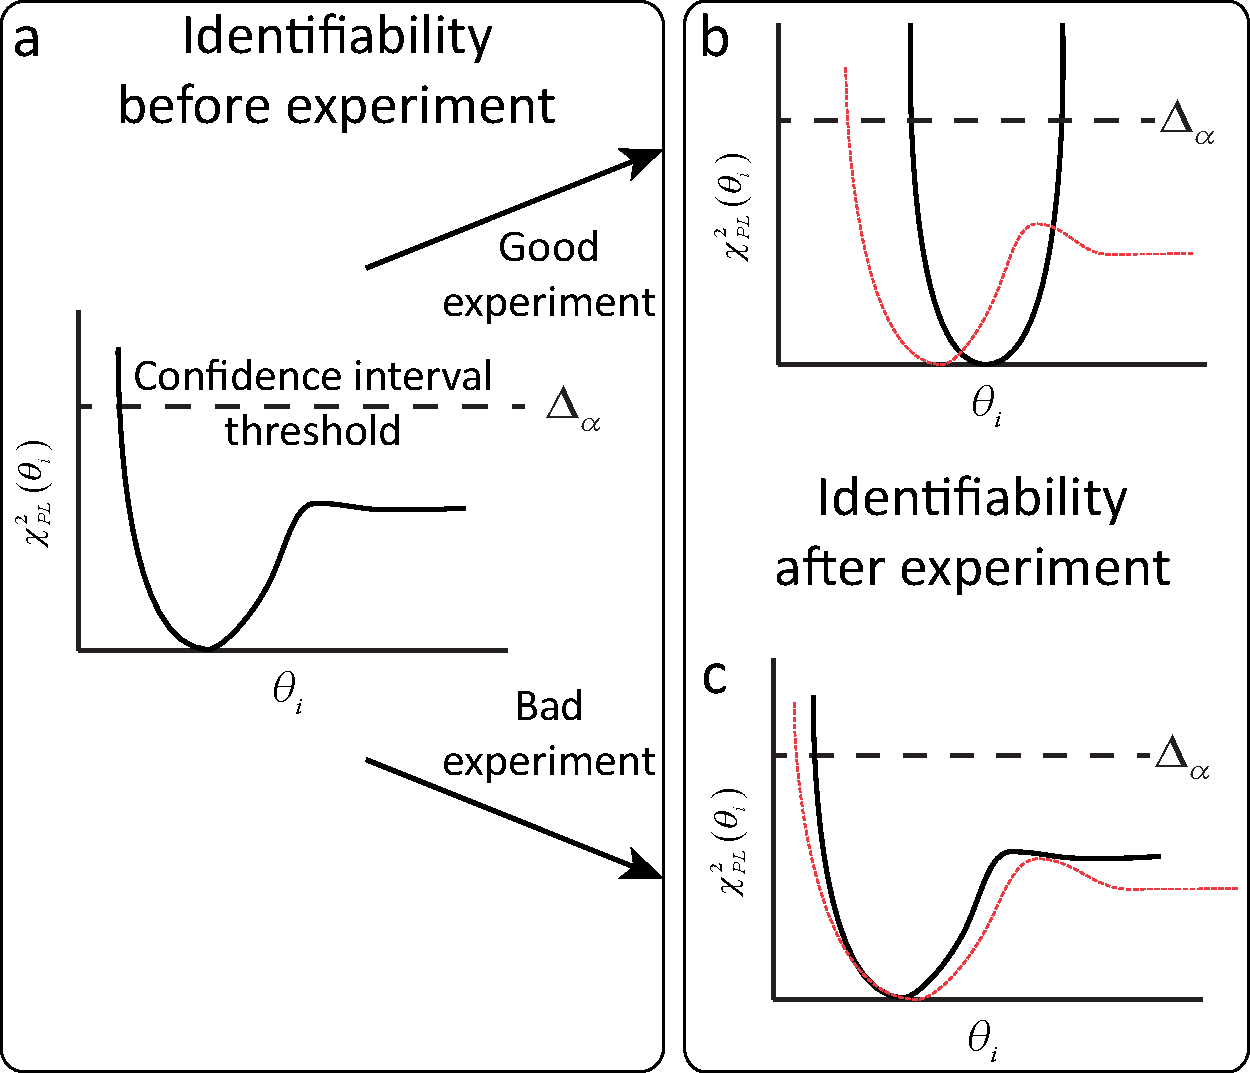
\includegraphics[width=.6\textwidth,height=.6\textheight,keepaspectratio]{figures/ed_with_pl}}
		\caption{Cartoon illustrating the utility of identifiability analysis for experimental design. a) The profile likelihood of a practically non-identifiable parameter that needs to be estimated based on both good and bad experimental data. The changes in the profile likelihood of the parameter when estimated with b) good experimental data and c) bad experimental. The practical identifiability of a parameter is dependent on the quality and quantity of experimental data used to estimate the parameter. The identifiability of the parameter, as determined using its profile likelihood, does not change due to the poor quality/quantity of experiments.}\label{fig:edwithpl}
	\end{figure}	
	
	\subsection{Identifiability analysis of parameters in a kinetic model of gluconeogenesis:}
	The proposed model for acetate consumption through gluconeogenesis and its corresponding kinetic model is used as a case study to illustrate the utility of identifiability analysis for the design of experiments for estimating parameters in kinetic models of metabolism. The kinetic model is described below.
	\begin{equation}\label{eq:ode1}
	\frac{d}{dt}pep=v_1-v_2-v_4
	\end{equation}
	\begin{equation}\label{eq:ode2}
	\frac{d}{dt}fdp=v_2-v_3
	\end{equation}
	\begin{equation}\label{eq:ode3}
	\frac{d}{dt}E=v_{e,max}\left(\frac{1}{1+\left(\frac{fdp}{K_{e}^{fdp}}\right)^{n_e}}\right) - d E
	\end{equation}
	The kinetic expressions for fluxes $v_1$ through $v_4$ are given below. The consumption of acetate through $v_1$ and conversion of \textit{pep} through $v_2$ are expressed in Equations (\ref{eq:flux1}) and (\ref{eq:flux2}) respectively using Michaelis-Menten kinetics. The acetate flux through $v_1$ is also governed by the quantity of available enzyme E. 
	\begin{equation}\label{eq:flux1}
	v_1 = k_{1}^{cat}E\frac{acetate}{acetate+K_{1}^{acetate}}
	\end{equation}	
	\begin{equation}\label{eq:flux2}
	v_2 = V_{2}^{max}\frac{pep}{pep+K_{2}^{pep}}
	\end{equation}
	\begin{equation}\label{eq:flux3}
	v_3 = V_{3}^{max}\frac{\tilde{fdp}\left(1+\tilde{fdp}\right)^3}{\left(1+\tilde{fdp}\right)^4+L_3\left(1+\frac{pep}{K_{3}^{pep}}\right)^{-4}}
	\end{equation}
	The allosterically regulated flux $v_3$ for the consumption of \textit{fdp} is expressed in Equation (\ref{eq:flux3}) using the Monod-Wyman-Changeux (MWC) model for allosterically regulated enzymes, where $\tilde{fdp}$ refers to the ratio of \textit{fdp} with respect to its allosteric binding constant $K_{3}^{fdp}$. The added flux $v_4$ for the export of \textit{pep} is expressed as a linear equation dependent on $pep$ in Equation (\ref{eq:flux4}).
	\begin{equation}\label{eq:flux4}
	v_4 = k_{4}^{cat}.pep
	\end{equation}
	
	\subsection{Parameter estimation in kinetic models of metabolism:}
	The formulation for parameter estimation assumes that the concentrations and the fluxes corresponding to each perturbation are variables in the optimization problem formulated to estimate kinetic parameters.
	
	Let $\mathbf{x}\in\mathbb{R}^m$, $\mathbf{p}\in\mathbb{R}^l$ and $\mathbf{v}\in\mathbb{R}$ be the vector of concentrations, parameters and fluxes respectively. If the number of perturbations used for parameter estimation is in $\mathbb{R}^p$, then the vector of concentrations, fluxes and parameters that need to be estimated in the optimization problem changes to $\mathbf{x}\in\mathbb{R}^{mp}, \mathbf{v}\in\mathbb{R}^{p}$ and $\mathbf{p}\in\mathbb{R}^{l}$ respectively. 
	
	Let $i\in\mathbb{R}^{mp}$, $j\in\mathbb{R}^{p}$ and $k\in\mathbb{R}^{l}$ represent the indices for concentrations, fluxes and parameters respectively in Equations (\ref{eq:l2norm-flux})-(\ref{eq:noise-var}).
	
	\paragraph{Formulation c):}
	In order to estimate kinetic parameters for fluxes in models of metabolism, we propose a formulation accounting for the uncertainty in the concentration and flux estimates. The uncertainty terms ($\epsilon$) are used as bounds for the flux and the concentrations and are included in the optimization objective as a variable to be penalized is given in Equation (\ref{eq:noise-var}) below. Note that the concentration and the fluxes have different uncertainties, $\epsilon_x$ and $\epsilon_v$ respectively, associated with them. $w_1$, $w_2$, $w_3$ and $w_4$ are the weights associated with the four different terms in the objective. 
	\begin{center}
		\begin{subequations}\label{eq:noise-var}
			\begin{align}
			\underset{\mathbf{x},\mathbf{p},\mathbf{v},\epsilon_x,\epsilon_v}{\mathrm{min}} & \text{      }w_1\left\Vert \mathbf{v}-\mathbf{v}^*\right\Vert + w_2\left\Vert \mathbf{x}-\mathbf{x}^*\right\Vert + w_3\epsilon_x + w_4\epsilon_v\\
			\mathrm{st}& \text{      }N(\mathbf{x},\mathbf{p}) - v_jD(\mathbf{x},\mathbf{p}) = 0 & \text{  }\forall & \text{ }j\in\mathbb{R}^p\\
			& \text{      }x^*_i(1-\epsilon_x)\le x_i \le x^*_i(1+\epsilon_x) & \text{  }\forall & \text{ }i\in\mathbb{R}^{mp}\\	
			& \text{      }v^*_j(1-\epsilon_v)\le v_j \le v^*_j(1+\epsilon_v) & \text{  }\forall & \text{ }j\in\mathbb{R}^{p}\\		
			& \text{      }\mathbf{p}_{min} \le \mathbf{p} \le \mathbf{p}_{max}
			\end{align}
		\end{subequations}
	\end{center}
	
	\begin{table}[!tbhp]
		\caption{Table showing the perturbed values of all fluxes used for parameter estimation.}
		\begin{center}				
			\begin{tabular}{ccc}
				Designation & Perturbed Fluxes & Perturbed Values\\
				\hline
				P1 & $v_1$ & 2\\
				P2 & $v_2$ & 0.2\\
				P3 & $v_3$ & 0.5
			\end{tabular}
		\end{center}	
		\label{tab:pval}
	\end{table}

	\section{Results:}

	\begin{table}[!tbhp]
		\caption{Table showing the ability of different formulations mentioned above to estimate enzyme kinetic parameters for different fluxes based on the perturbations given in the above table.}
		\begin{center}				
			\begin{tabular}{cccccc}
				\hline
				Flux & Data Type & \multicolumn{2}{c}{Formulation (b)} & \multicolumn{2}{c}{Formulation (c)}\\
				\hline
				&&$\epsilon_x$(\%)&$\epsilon_v$(\%)&$\epsilon_x$(\%)&$\epsilon_v$(\%)\\
				\hline
				\multirow{2}{*}{flux 1} & no noise & 30 & 5 & 33.33 & 0\\
												  &	noisy & x & x & 0 & 33.33\\
			  	\hline
				 \multirow{2}{*}{flux 2} & no noise & 90 & 30 & 0 & 31\\
				 									& noisy & 85 & 40 & 0 & 30\\
				\hline				 									
				\multirow{2}{*}{flux 3} & no noise & 15 & 10 & 17 & 0\\
													& noisy & x & x & 17 & 0\\
				\hline			
			\end{tabular}
		\end{center}	
		\label{tab:res1}
	\end{table}
	\subsection{Estimation of flux 1:}
	\begin{figure}[!tbhp]
		\centering{\includegraphics[width=.5\textwidth,height=.5\textheight,keepaspectratio]{C:/Users/shyam/Documents/Courses/CHE1125Project/Results/estimation/est_flux1/no_noise/typec/est_flux1_conc_aug6}}
		\caption{Plot comparing noiseless model generated steady state metabolite concentrations with model estimates obtained using an optimized model for $v_1$ using formulation (c). }
	\end{figure}
	\begin{figure}[!tbhp]
		\centering{\includegraphics[width=.5\textwidth,height=.5\textheight,keepaspectratio]{C:/Users/shyam/Documents/Courses/CHE1125Project/Results/estimation/est_flux1/noisy/typec/est_flux1_conc_aug6}}
		\caption{Plot comparing noisy model generated steady state metabolite concentrations with model estimates obtained using an optimized model for $v_1$ using formulation (c). }
	\end{figure}
	\begin{figure}[!tbhp]
		\centering{\includegraphics[width=.5\textwidth,height=.5\textheight,keepaspectratio]{C:/Users/shyam/Documents/Courses/CHE1125Project/Results/estimation/est_flux1/no_noise/typec/est_flux1_flux_aug6}}
		\caption{Plot comparing noiseless model generated steady state fluxes with model estimates obtained using an optimized model for $v_1$ using formulation (c). }
	\end{figure}
	\begin{figure}[!tbhp]
		\centering{\includegraphics[width=.5\textwidth,height=.5\textheight,keepaspectratio]{C:/Users/shyam/Documents/Courses/CHE1125Project/Results/estimation/est_flux1/noisy/typec/est_flux1_flux_aug6}}
		\caption{Plot comparing noisy model generated steady state fluxes with model estimates obtained using an optimized model for $v_1$ using formulation (c). }
	\end{figure}
	\begin{figure}[!tbhp]
		\centering{\includegraphics[width=.5\textwidth,height=.5\textheight,keepaspectratio]{C:/Users/shyam/Documents/Courses/CHE1125Project/Results/estimation/est_flux1/no_noise/typec/est_flux1_par_aug6}}
		\caption{Plot comparing noiseless model generated parameters for $v_1$ through a multi-start search algorithm using formulation (c). }
	\end{figure}
	\begin{figure}[!tbhp]
		\centering{\includegraphics[width=.5\textwidth,height=.5\textheight,keepaspectratio]{C:/Users/shyam/Documents/Courses/CHE1125Project/Results/estimation/est_flux1/noisy/typec/est_flux1_par_aug6}}
		\caption{Plot comparing noisy model generated parameters for $v_1$ through a multi-start search algorithm using formulation (c). }
	\end{figure}
	\clearpage

	\subsection{Estimation of flux 2:}
	\begin{figure}[!tbhp]
		\centering{\includegraphics[width=.5\textwidth,height=.5\textheight,keepaspectratio]{C:/Users/shyam/Documents/Courses/CHE1125Project/Results/estimation/est_flux2/no_noise/typec/est_flux2_conc_aug6}}
		\caption{Plot comparing noiseless model generated steady state metabolite concentrations with model estimates obtained using an optimized model for $v_2$ using formulation (c). }
	\end{figure}
	\begin{figure}[!tbhp]
		\centering{\includegraphics[width=.5\textwidth,height=.5\textheight,keepaspectratio]{C:/Users/shyam/Documents/Courses/CHE1125Project/Results/estimation/est_flux2/noisy/typec/est_flux2_conc_aug6}}
		\caption{Plot comparing noisy model generated steady state metabolite concentrations with model estimates obtained using an optimized model for $v_2$ using formulation (c). }
	\end{figure}
	\begin{figure}[!tbhp]
		\centering{\includegraphics[width=.5\textwidth,height=.5\textheight,keepaspectratio]{C:/Users/shyam/Documents/Courses/CHE1125Project/Results/estimation/est_flux2/no_noise/typec/est_flux2_flux_aug6}}
		\caption{Plot comparing noiseless model generated steady state fluxes with model estimates obtained using an optimized model for $v_2$ using formulation (c). }
	\end{figure}
	\begin{figure}[!tbhp]
		\centering{\includegraphics[width=.5\textwidth,height=.5\textheight,keepaspectratio]{C:/Users/shyam/Documents/Courses/CHE1125Project/Results/estimation/est_flux2/noisy/typec/est_flux2_flux_aug6}}
		\caption{Plot comparing noisy model generated steady state fluxes with model estimates obtained using an optimized model for $v_2$ using formulation (c). }
	\end{figure}
	\begin{figure}[!tbhp]
		\centering{\includegraphics[width=.5\textwidth,height=.5\textheight,keepaspectratio]{C:/Users/shyam/Documents/Courses/CHE1125Project/Results/estimation/est_flux2/no_noise/typec/est_flux2_par_aug6}}
		\caption{Plot comparing noiseless model generated parameters for $v_2$ through a multi-start search algorithm using formulation (c). }
	\end{figure}
	\begin{figure}[!tbhp]
		\centering{\includegraphics[width=.5\textwidth,height=.5\textheight,keepaspectratio]{C:/Users/shyam/Documents/Courses/CHE1125Project/Results/estimation/est_flux2/noisy/typec/est_flux2_par_aug6}}
		\caption{Plot comparing noisy model generated parameters for $v_2$ through a multi-start search algorithm using formulation (c). }
	\end{figure}
	\clearpage
	
	\subsection{Estimation of flux 3:}
	\begin{figure}[!tbhp]
		\centering{\includegraphics[width=.5\textwidth,height=.5\textheight,keepaspectratio]{C:/Users/shyam/Documents/Courses/CHE1125Project/Results/estimation/est_flux3/no_noise/typec/est_flux3_conc_aug6}}
		\caption{Plot comparing noiseless model generated steady state metabolite concentrations with model estimates obtained using an optimized model for $v_3$ using formulation (c). }
	\end{figure}
	\begin{figure}[!tbhp]
		\centering{\includegraphics[width=.5\textwidth,height=.5\textheight,keepaspectratio]{C:/Users/shyam/Documents/Courses/CHE1125Project/Results/estimation/est_flux3/noisy/typec/est_flux3_conc_aug6}}
		\caption{Plot comparing noisy model generated steady state metabolite concentrations with model estimates obtained using an optimized model for $v_3$ using formulation (c). }
	\end{figure}
	\begin{figure}[!tbhp]
		\centering{\includegraphics[width=.5\textwidth,height=.5\textheight,keepaspectratio]{C:/Users/shyam/Documents/Courses/CHE1125Project/Results/estimation/est_flux3/no_noise/typec/est_flux3_flux_aug6}}
		\caption{Plot comparing noiseless model generated steady state fluxes with model estimates obtained using an optimized model for $v_3$ using formulation (c). }
	\end{figure}
	\begin{figure}[!tbhp]
		\centering{\includegraphics[width=.5\textwidth,height=.5\textheight,keepaspectratio]{C:/Users/shyam/Documents/Courses/CHE1125Project/Results/estimation/est_flux3/noisy/typec/est_flux3_flux_aug6}}
		\caption{Plot comparing noisy model generated steady state fluxes with model estimates obtained using an optimized model for $v_3$ using formulation (c). }
	\end{figure}
	\begin{figure}[!tbhp]
		\centering{\includegraphics[width=.5\textwidth,height=.5\textheight,keepaspectratio]{C:/Users/shyam/Documents/Courses/CHE1125Project/Results/estimation/est_flux3/no_noise/typec/est_flux3_par_aug6}}
		\caption{Plot comparing noiseless model generated parameters for $v_3$ through a multi-start search algorithm using formulation (c). }
	\end{figure}
	\begin{figure}[!tbhp]
		\centering{\includegraphics[width=.5\textwidth,height=.5\textheight,keepaspectratio]{C:/Users/shyam/Documents/Courses/CHE1125Project/Results/estimation/est_flux3/noisy/typec/est_flux3_par_aug6}}
		\caption{Plot comparing noisy model generated parameters for $v_3$ through a multi-start search algorithm using formulation (c). }
	\end{figure}
	\clearpage
	
	\section{Appendix}
	\subsection{Formulation a):}		
	\begin{subequations}\label{eq:l2norm-flux}
		\begin{align}
		\underset{\mathbf{x},\mathbf{p},\mathbf{v}}{\mathrm{min}} & \text{      }\left\Vert \mathbf{v}-\mathbf{v}^*\right\Vert\\
		\mathrm{st}& \text{      }N(\mathbf{x},\mathbf{p}) - v_jD(\mathbf{x},\mathbf{p}) = 0 & \text{  }\forall & \text{ }j\in\mathbb{R}^p\\
		& \text{      }x^*_i(1-\epsilon)\le x_i \le x^*_i(1+\epsilon) & \text{  }\forall & \text{ }i\in\mathbb{R}^{mp}\\	
		& \text{      }v^*_j(1-\epsilon)\le v_j \le v^*_j(1+\epsilon) & \text{  }\forall & \text{ }j\in\mathbb{R}^{p}\\		
		& \text{      }\mathbf{p}_{min} \le \mathbf{p} \le \mathbf{p}_{max}
		\end{align}
	\end{subequations}
	
	\subsection{Formulation b):}	
	In this formulation, in Equation (\ref{eq:l2norm-conc}), the flux and concentrations are constrained as earlier with an uncertainty term.	
	\begin{subequations}\label{eq:l2norm-conc}
		\begin{align}
		\underset{\mathbf{x},\mathbf{p},\mathbf{v}}{\mathrm{min}} & \text{      }w_1\left\Vert \mathbf{v}-\mathbf{v}^*\right\Vert + w_2\left\Vert \mathbf{x}-\mathbf{x}^*\right\Vert\\
		\mathrm{st}& \text{      }N(\mathbf{x},\mathbf{p}) - v_jD(\mathbf{x},\mathbf{p}) = 0 & \text{  }\forall & \text{ }j\in\mathbb{R}^p\\
		& \text{      }x^*_i(1-\epsilon)\le x_i \le x^*_i(1+\epsilon) & \text{  }\forall & \text{ }i\in\mathbb{R}^{mp}\\	
		& \text{      }v^*_j(1-\epsilon)\le v_j \le v^*_j(1+\epsilon) & \text{  }\forall & \text{ }j\in\mathbb{R}^{p}\\		
		& \text{      }\mathbf{p}_{min} \le \mathbf{p} \le \mathbf{p}_{max}
		\end{align}
	\end{subequations}	
	
	\subsection{Formulation d):}
	Due to the inability of Equation (\ref{eq:l2norm-flux}) to get feasible results, we modified the problem to include the L2-norm of the concentrations as well in the objective function in Equation (\ref{eq:free-var}a). In Equation (\ref{eq:free-var}) the flux and the concentrations are free variables, i.e.,  $\mathbf{x}\in\left[\mathbf{0},+\mathbf{\infty}\right]$. 
	\begin{subequations}\label{eq:free-var}
		\begin{align}
		\underset{\mathbf{x},\mathbf{p},\mathbf{v}}{\mathrm{min}} & \text{      }w_1\left\Vert \mathbf{v}-\mathbf{v}^*\right\Vert + w_2\left\Vert \mathbf{x}-\mathbf{x}^*\right\Vert\\
		\mathrm{st}& \text{      }N(\mathbf{x},\mathbf{p}) - v_jD(\mathbf{x},\mathbf{p}) = 0 & \text{  }\forall & \text{ }j\in\mathbb{R}^p\\
		& \text{      }0\le x_i \le +\infty & \text{  }\forall & \text{ }i\in\mathbb{R}^{mp}\\	
		& \text{      }0\le v_j \le +\infty & \text{  }\forall & \text{ }j\in\mathbb{R}^{p}\\		
		& \text{      }\mathbf{p}_{min} \le \mathbf{p} \le \mathbf{p}_{max}
		\end{align}
	\end{subequations}
	
	After testing the problem in Equation (\ref{eq:free-var}) above for the acetate uptake flux $v_1$, we found that all solutions using IPOPT exceeded the maximum number of iterations (set at 5000) and never produced an optimal solution. Hence, we use a modified form of the bounds in Equation (\ref{eq:free-var}) above in Equation (\ref{eq:l2norm-conc}).
	
	\printbibliography
\end{document}